\documentclass[]{article}
\usepackage{lmodern}
\usepackage{amssymb,amsmath}
\usepackage{ifxetex,ifluatex}
\usepackage{fixltx2e} % provides \textsubscript
\ifnum 0\ifxetex 1\fi\ifluatex 1\fi=0 % if pdftex
  \usepackage[T1]{fontenc}
  \usepackage[utf8]{inputenc}
\else % if luatex or xelatex
  \ifxetex
    \usepackage{mathspec}
  \else
    \usepackage{fontspec}
  \fi
  \defaultfontfeatures{Ligatures=TeX,Scale=MatchLowercase}
\fi
% use upquote if available, for straight quotes in verbatim environments
\IfFileExists{upquote.sty}{\usepackage{upquote}}{}
% use microtype if available
\IfFileExists{microtype.sty}{%
\usepackage{microtype}
\UseMicrotypeSet[protrusion]{basicmath} % disable protrusion for tt fonts
}{}
\usepackage[margin=1in]{geometry}
\usepackage{hyperref}
\hypersetup{unicode=true,
            pdftitle={DATA 605 - Final Exam},
            pdfauthor={Joshua Sturm},
            pdfborder={0 0 0},
            breaklinks=true}
\urlstyle{same}  % don't use monospace font for urls
\usepackage{graphicx,grffile}
\makeatletter
\def\maxwidth{\ifdim\Gin@nat@width>\linewidth\linewidth\else\Gin@nat@width\fi}
\def\maxheight{\ifdim\Gin@nat@height>\textheight\textheight\else\Gin@nat@height\fi}
\makeatother
% Scale images if necessary, so that they will not overflow the page
% margins by default, and it is still possible to overwrite the defaults
% using explicit options in \includegraphics[width, height, ...]{}
\setkeys{Gin}{width=\maxwidth,height=\maxheight,keepaspectratio}
\IfFileExists{parskip.sty}{%
\usepackage{parskip}
}{% else
\setlength{\parindent}{0pt}
\setlength{\parskip}{6pt plus 2pt minus 1pt}
}
\setlength{\emergencystretch}{3em}  % prevent overfull lines
\providecommand{\tightlist}{%
  \setlength{\itemsep}{0pt}\setlength{\parskip}{0pt}}
\setcounter{secnumdepth}{0}
% Redefines (sub)paragraphs to behave more like sections
\ifx\paragraph\undefined\else
\let\oldparagraph\paragraph
\renewcommand{\paragraph}[1]{\oldparagraph{#1}\mbox{}}
\fi
\ifx\subparagraph\undefined\else
\let\oldsubparagraph\subparagraph
\renewcommand{\subparagraph}[1]{\oldsubparagraph{#1}\mbox{}}
\fi

%%% Use protect on footnotes to avoid problems with footnotes in titles
\let\rmarkdownfootnote\footnote%
\def\footnote{\protect\rmarkdownfootnote}

%%% Change title format to be more compact
\usepackage{titling}

% Create subtitle command for use in maketitle
\newcommand{\subtitle}[1]{
  \posttitle{
    \begin{center}\large#1\end{center}
    }
}

\setlength{\droptitle}{-2em}
  \title{DATA 605 - Final Exam}
  \pretitle{\vspace{\droptitle}\centering\huge}
  \posttitle{\par}
  \author{Joshua Sturm}
  \preauthor{\centering\large\emph}
  \postauthor{\par}
  \predate{\centering\large\emph}
  \postdate{\par}
  \date{May 17, 2018}


\begin{document}
\maketitle

\hypertarget{kaggle-data}{%
\section{1. Kaggle Data}\label{kaggle-data}}

You are to register for Kaggle.com (free) and compete in the House
Prices: Advanced Regression Techniques competition.
\url{https://www.kaggle.com/c/house-prices-advanced-regression-techniques}.
I want you to do the following

\begin{itemize}
\item
  Pick one of the quantitative independent variables from the training
  data set (train.csv), and define that variable as X. Make sure this
  variable is skewed to the right!
\item
  Pick the dependent variable and define it as Y.
\end{itemize}

Since the requirement is to pick an independent variables that is skewed
to the right, I'll begin by plotting a histogram for each (numeric)
variable.

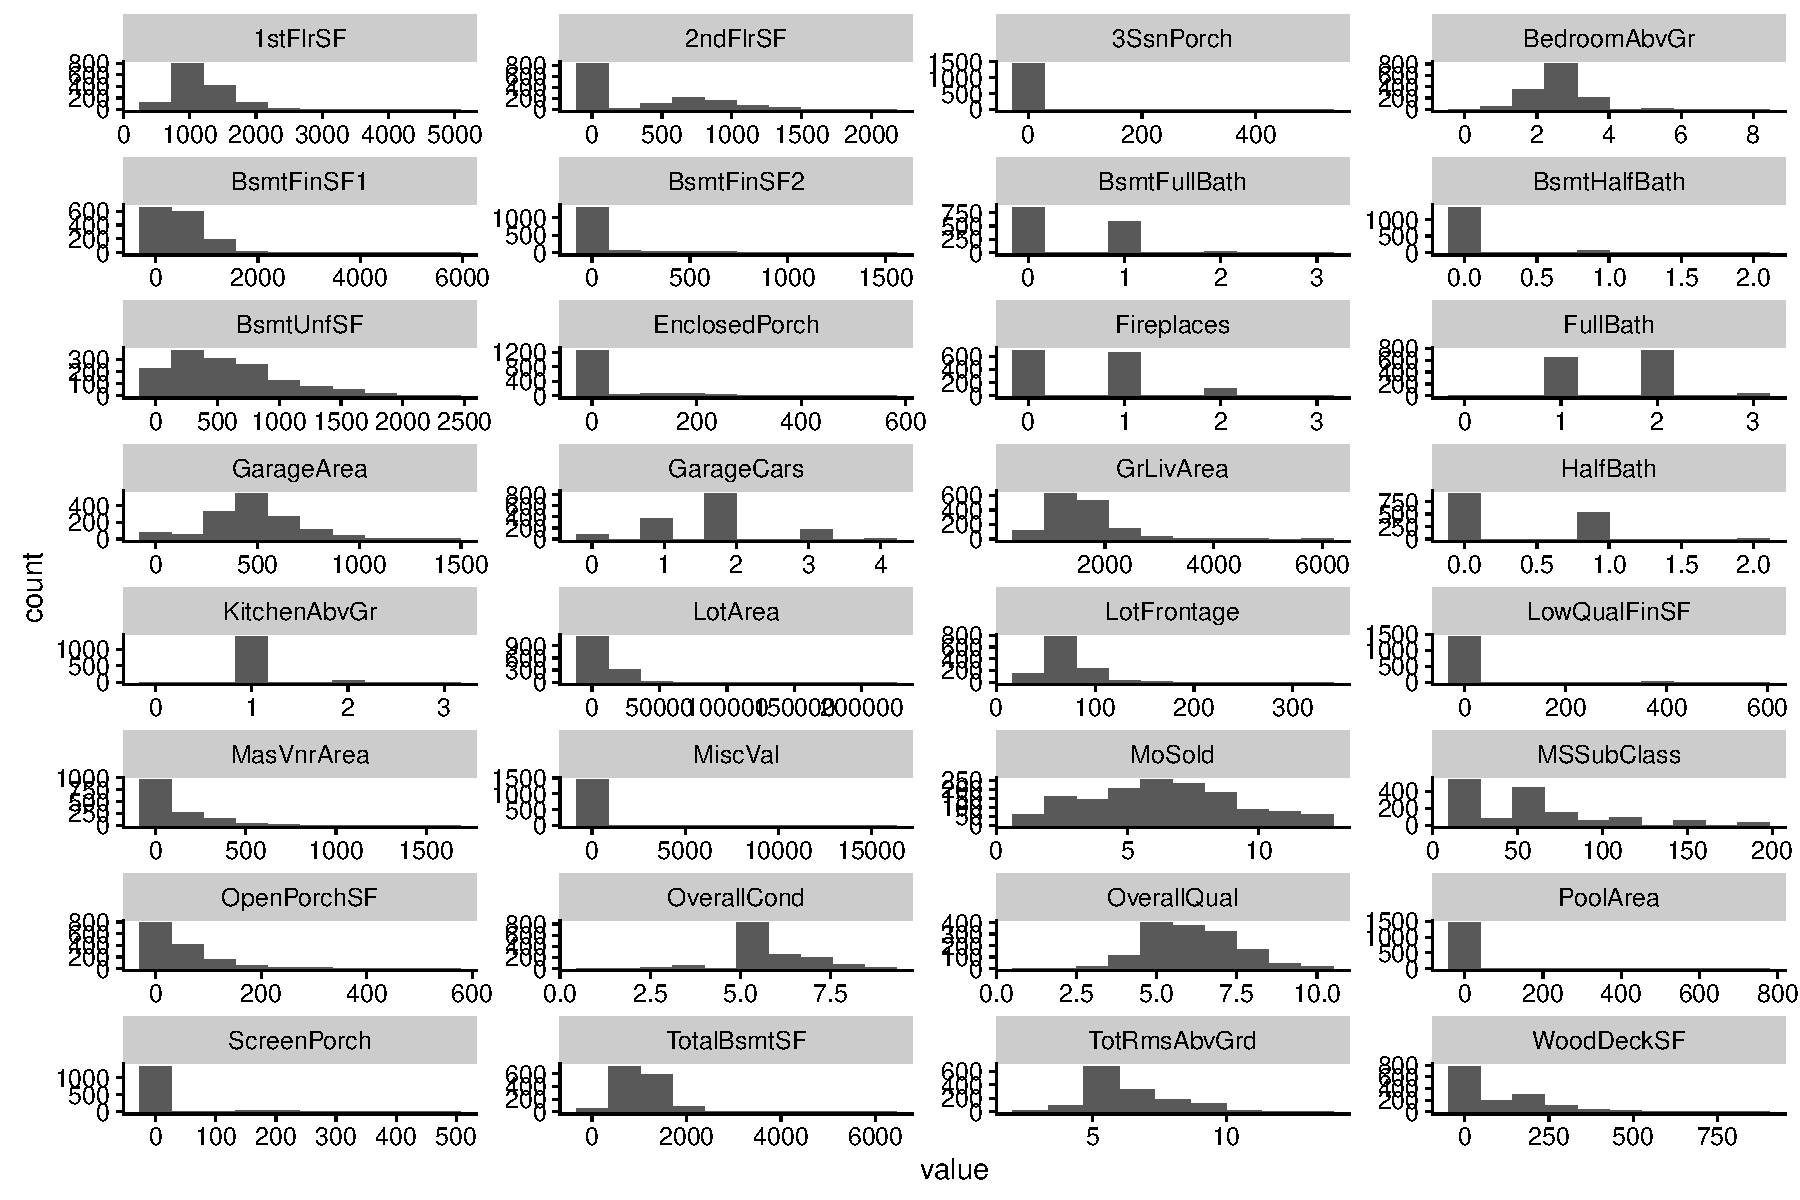
\includegraphics{DATA_605_Final_Exam_files/figure-latex/train-histogram-1.pdf}

I'm going to use \texttt{OpenPorchSF} as my independent variable. Of
course, since we're trying to predict the house's sale price,
\texttt{SalePrice} will be the dependent variable.

\hypertarget{probability}{%
\section{2. Probability}\label{probability}}

Calculate as a minimum the below probabilities a through c. Assume the
small letter ``x'' is estimated as the 1st quartile of the X variable,
and the small letter ``y'' is estimated as the 1st quartile of the Y
variable. Interpret the meaning of all probabilities. In addition, make
a table of counts as shown below.

\begin{center}
a. $P(X > x | Y > y)$  \hspace{20pt} b. $P(X > x, Y > Y)$ \hspace{20pt} c. $P(X < x | Y > y)$
\end{center}

~ ~

\hypertarget{a.}{%
\subsection{a.}\label{a.}}

\[
P(X > x | Y > y) = \frac{P(X > x \cap Y > y)}{P(Y > y)}
\]

In words, we're looking for the conditional probability that the
\texttt{OpenPorchSF} variable is greater than its first quantile,
\textbf{given} that \texttt{SalePrice} is greather than its first
quantile.

\begin{verbatim}
## [1] "Probability = 0.647488584474886"
\end{verbatim}

\hypertarget{b.}{%
\subsection{b.}\label{b.}}

\[
P(X > x, Y > Y) = P(X > x \cap Y > y)
\]

\begin{verbatim}
## [1] "Probability = 0.485616438356164"
\end{verbatim}

\hypertarget{c.}{%
\subsection{c.}\label{c.}}

\[
P(X < x | Y > y) = \frac{P(X < x \cap Y > y)}{P(Y > y)}
\]

\begin{verbatim}
## [1] "Probability = 0"
\end{verbatim}

\begin{center}
\begin{tabular}{|c|c|c|c|}
\hline
x/y & $\leq$ 1st quartile & $>$ 1st quartile & Total \\ \hline
$\leq$ 1st quartile & 270 & 386 & 656 \\ \hline
$>$ 1st quartile & 95  &  709 & 804 \\ \hline
Total & 365 & 1095 & 1460 \\ \hline
\end{tabular}
\end{center}

\hypertarget{independence}{%
\subsection{2.2 Independence}\label{independence}}

Does splitting the training data in this fashion make them independent?
Let A be the new variable counting those observations above the 1st
quartile for X, and let B be the new variable counting those
observations above the 1st quartile for Y. Does P(AB)=P(A)P(B)? Check
mathematically, and then evaluate by running a Chi Square test for
association.

\begin{verbatim}
## [1] "A = 804"
## [1] "B = 1095"
## [1] "P(A) = 0.550684931506849"
## [1] "P(B) = 0.75"
## [1] "P(A)P(B) = 0.413013698630137"
## [1] "P(AB) = 0.485616438356164"
## [1] "Mean relative difference: 0.1757877"
\end{verbatim}

We can see that the two are not equal, that is,
\(P(AB) \neq P(A)\times P(B)\). So we've shown mathematically that
they're not independent.

\begin{verbatim}
## 
##  Pearson's Chi-squared test
## 
## data:  train$OpenPorchSF and train$SalePrice
## X-squared = 144030, df = 133060, p-value < 2.2e-16
\end{verbatim}

With a p-value \textless{} 0.05, we can reject the null hypothesis that
the variables are independent, and conclude that they are dependent.

\hypertarget{descriptive-and-inferential-statistics}{%
\section{3. Descriptive and Inferential
Statistics}\label{descriptive-and-inferential-statistics}}

Provide univariate descriptive statistics and appropriate plots for the
training data set. Provide a scatterplot of X and Y. Derive a
correlation matrix for any THREE quantitative variables in the dataset.
Test the hypotheses that the correlations between each pairwise set of
variables is 0 and provide a 92\% confidence interval. Discuss the
meaning of your analysis. Would you be worried about familywise error?
Why or why not?

For brevity's sake, I'll only summarize the last 10 (numeric) columns.

\begin{verbatim}
##               vars    n      mean       sd median   trimmed      mad   min
## WoodDeckSF      29 1460     94.24   125.34      0     71.76     0.00     0
## OpenPorchSF     30 1460     46.66    66.26     25     33.23    37.06     0
## EnclosedPorch   31 1460     21.95    61.12      0      3.87     0.00     0
## 3SsnPorch       32 1460      3.41    29.32      0      0.00     0.00     0
## ScreenPorch     33 1460     15.06    55.76      0      0.00     0.00     0
## PoolArea        34 1460      2.76    40.18      0      0.00     0.00     0
## MiscVal         35 1460     43.49   496.12      0      0.00     0.00     0
## MoSold          36 1460      6.32     2.70      6      6.25     2.97     1
## YrSold          37 1460   2007.82     1.33   2008   2007.77     1.48  2006
## SalePrice       38 1460 180921.20 79442.50 163000 170783.29 56338.80 34900
##                  max  range  skew kurtosis      se
## WoodDeckSF       857    857  1.54     2.97    3.28
## OpenPorchSF      547    547  2.36     8.44    1.73
## EnclosedPorch    552    552  3.08    10.37    1.60
## 3SsnPorch        508    508 10.28   123.06    0.77
## ScreenPorch      480    480  4.11    18.34    1.46
## PoolArea         738    738 14.80   222.19    1.05
## MiscVal        15500  15500 24.43   697.64   12.98
## MoSold            12     11  0.21    -0.41    0.07
## YrSold          2010      4  0.10    -1.19    0.03
## SalePrice     755000 720100  1.88     6.50 2079.11
\end{verbatim}

I've already plotted histograms in \protect\hyperlink{kaggle-data}{part
1}. I will do boxplots for numeric variables, and bar charts for
categorical data.

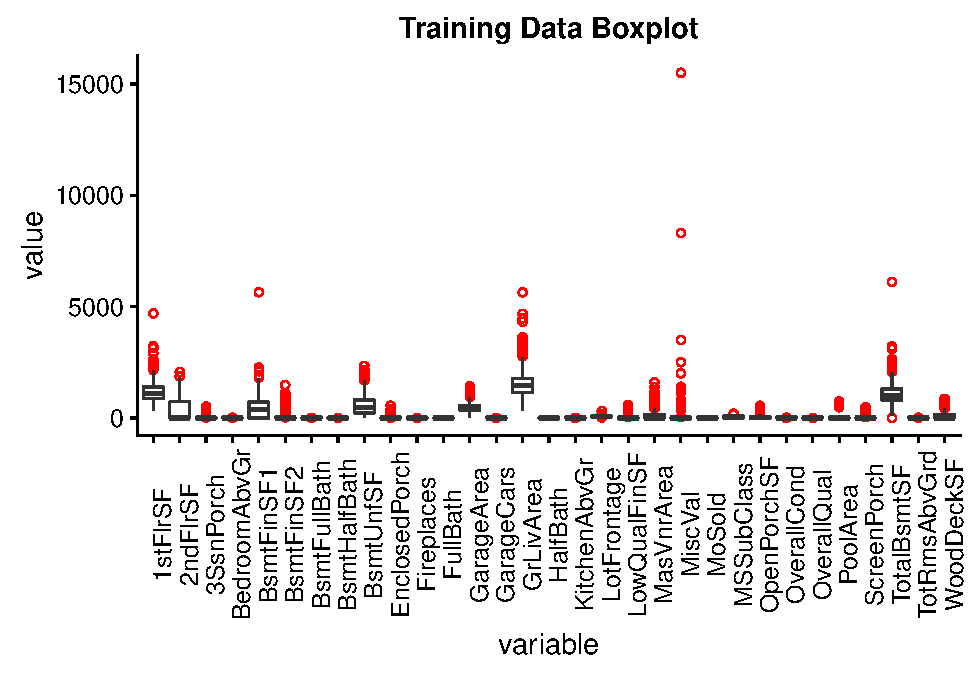
\includegraphics{DATA_605_Final_Exam_files/figure-latex/boxplots-1.pdf}

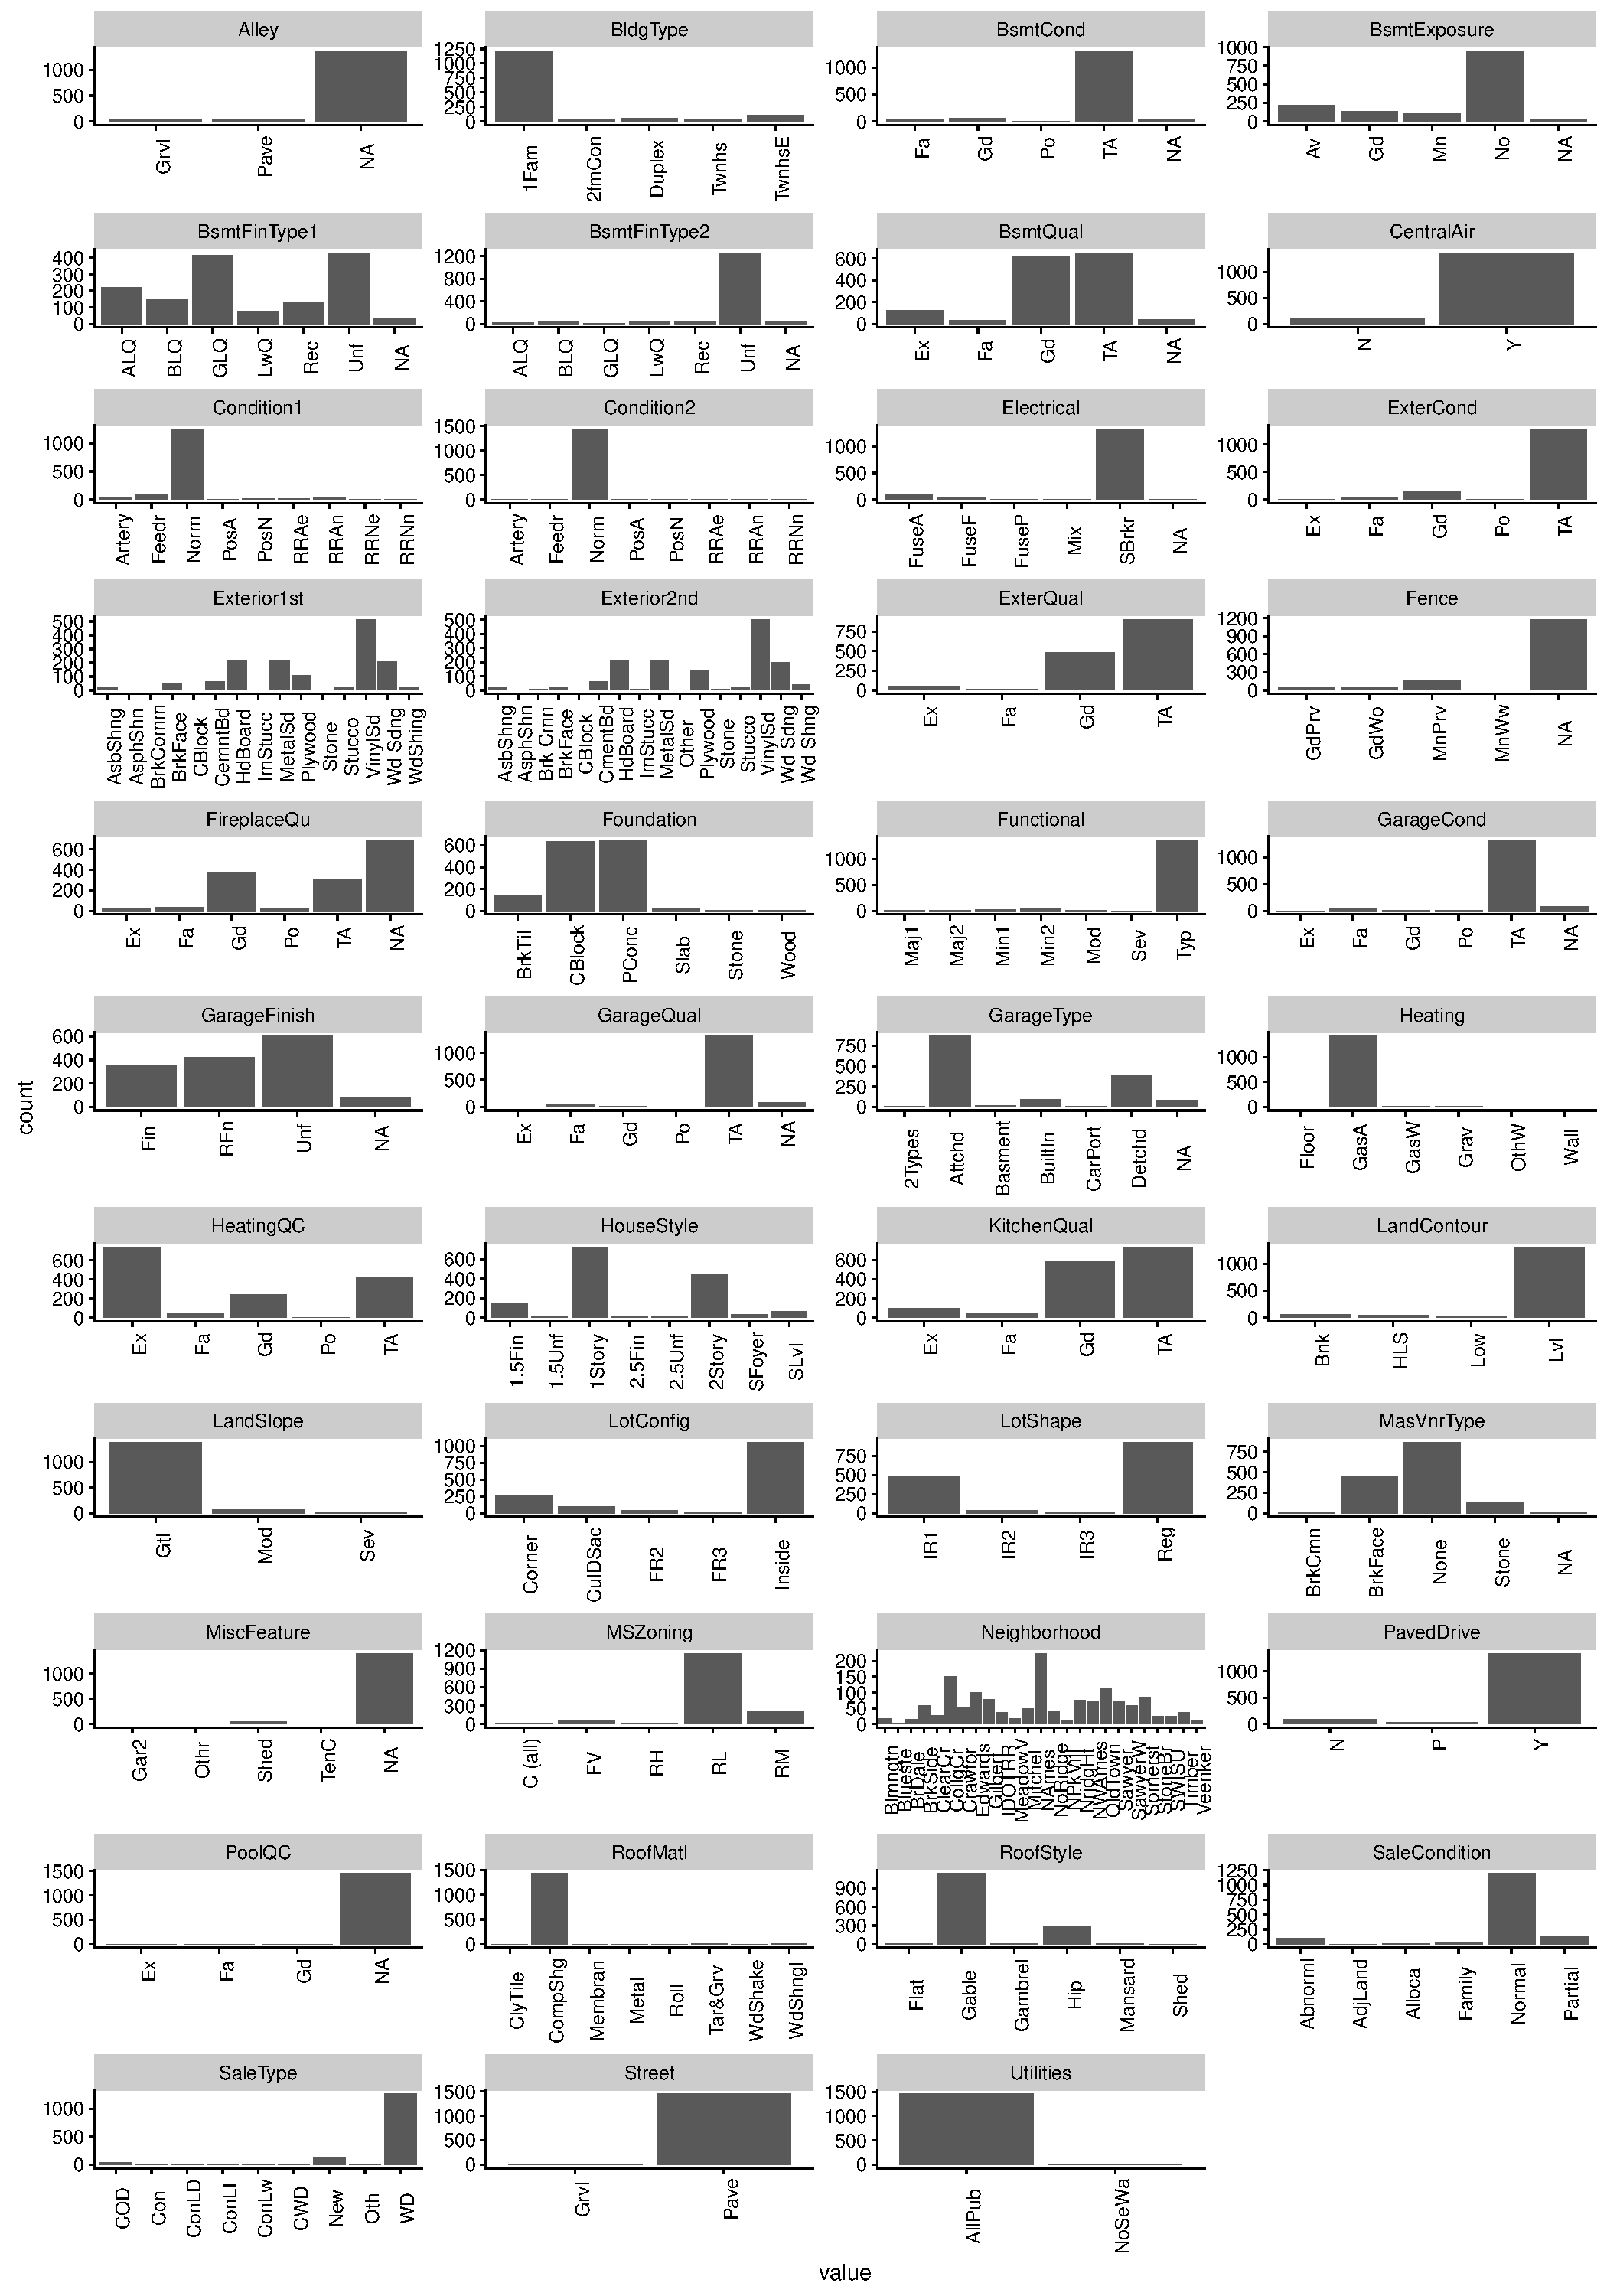
\includegraphics{DATA_605_Final_Exam_files/figure-latex/bar-charts-1.pdf}

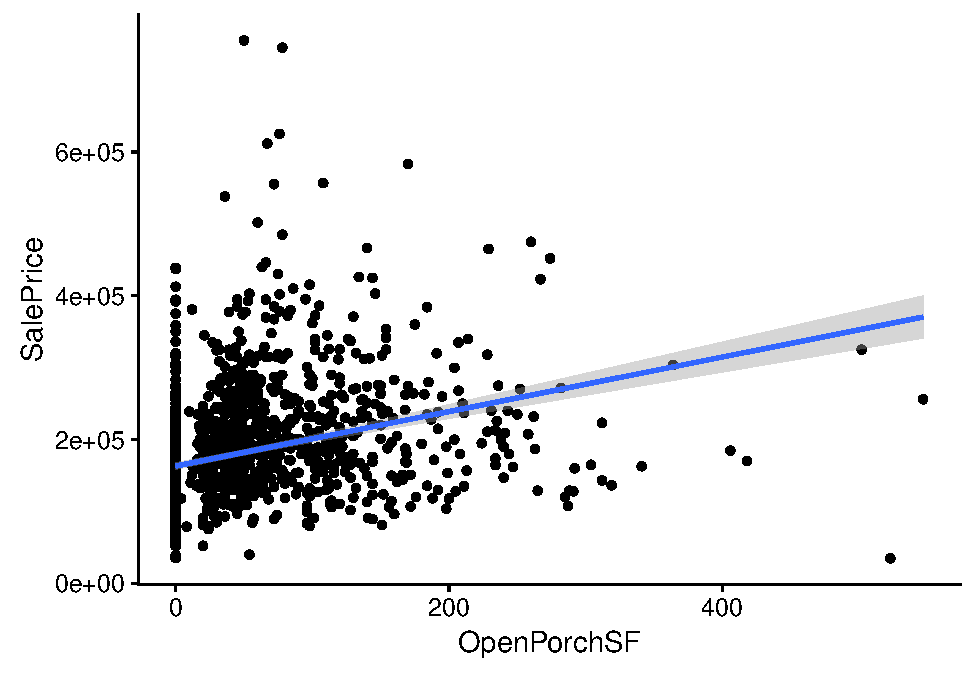
\includegraphics{DATA_605_Final_Exam_files/figure-latex/scatter-xy-1.pdf}

\(H_0:\) The correlation coefficient is 0, which is to say that these
variables aren't related. \(H_1:\) The correlation coefficient is not 0.

\begin{verbatim}
## 
##  Pearson's product-moment correlation
## 
## data:  train$MSSubClass and train$firstFlrSF
## t = -9.933, df = 1458, p-value < 2.2e-16
## alternative hypothesis: true correlation is not equal to 0
## 92 percent confidence interval:
##  -0.2941963 -0.2083297
## sample estimates:
##        cor 
## -0.2517584
## 
##  Pearson's product-moment correlation
## 
## data:  train$MSSubClass and train$GrLivArea
## t = 2.8662, df = 1458, p-value = 0.004214
## alternative hypothesis: true correlation is not equal to 0
## 92 percent confidence interval:
##  0.02912052 0.12027312
## sample estimates:
##        cor 
## 0.07485318
## 
##  Pearson's product-moment correlation
## 
## data:  train$firstFlrSF and train$GrLivArea
## t = 26.217, df = 1458, p-value < 2.2e-16
## alternative hypothesis: true correlation is not equal to 0
## 92 percent confidence interval:
##  0.5340458 0.5963849
## sample estimates:
##      cor 
## 0.566024
\end{verbatim}

Since the p-value for all three tests is much smaller than
\(\alpha = 0.08\), we can reject the null hypothesis, and conclude that
there is some correlation between the variables.

According to
\href{https://en.wikipedia.org/wiki/Family-wise_error_rate}{this
wikipedia article}, familywise error is a type 1 error, which occurs
when one rejects a true null hypothesis (aka a false positive). The
probability of making one or more of these can be controlled by ensuring
\[
FWER = P(V \geq 1) = 1 - P(v = 0) \leq \alpha
\]

\(FWER = 1-(1-0.08)^3 =\) 0.221312

So we should proceed with caution, since there is a
\textasciitilde{}22\% chance of making a type 1 error.

\hypertarget{linear-algebra-and-correlation}{%
\section{4. Linear Algebra and
Correlation}\label{linear-algebra-and-correlation}}

Invert your \(3 \times 3\) correlation matrix from above. (This is known
as the precision matrix and contains variance inflation factors on the
diagonal.) Multiply the correlation matrix by the precision matrix, and
then multiply the precision matrix by the correlation matrix. Conduct LU
decomposition on the matrix.

Invert our correlation matrix

Multiplying the correlation matrix by the precision (inverted) matrix

\begin{verbatim}
##            MSSubClass firstFlrSF GrLivArea
## MSSubClass          1          0         0
## firstFlrSF          0          1         0
## GrLivArea           0          0         1
##            MSSubClass firstFlrSF GrLivArea
## MSSubClass          1          0         0
## firstFlrSF          0          1         0
## GrLivArea           0          0         1
\end{verbatim}

The result of the matrix multiplcation is the identity matrix.

To perform the LU decomposition, I'll recycle the function I created for
assignment 2.

\begin{verbatim}
## [[1]]
##             [,1]      [,2] [,3]
## [1,]  1.00000000 0.0000000    0
## [2,] -0.25175835 1.0000000    0
## [3,]  0.07485318 0.6244478    1
## 
## [[2]]
##            MSSubClass firstFlrSF  GrLivArea
## MSSubClass          1 -0.2517584 0.07485318
## firstFlrSF          0  0.9366177 0.58486888
## GrLivArea           0  0.0000000 0.62917691
\end{verbatim}

\hypertarget{calculus-based-probability-statistics}{%
\section{5. Calculus-Based Probability \&
Statistics}\label{calculus-based-probability-statistics}}

Many times, it makes sense to fit a closed form distribution to data.
For the first variable that you selected which is skewed to the right,
shift it so that the minimum value is above zero as necessary. Then load
the MASS package and run fitdistr to fit an exponential probability
density function. (See
\url{https://stat.ethz.ch/R-manual/R-devel/library/MASS/html/fitdistr.html}
). Find the optimal value of \(\lambda\) for this distribution, and then
take 1000 samples from this exponential distribution using this value
(e.g., rexp(1000, \(\lambda\))). Plot a histogram and compare it with a
histogram of your original variable. Using the exponential pdf, find the
5th and 95th percentiles using the cumulative distribution function
(CDF). Also generate a 95\% confidence interval from the empirical data,
assuming normality. Finally, provide the empirical 5th percentile and
95th percentile of the data. Discuss.

Since the minimum \texttt{OpenPorchSF} value is 0, I'll shift it to the
right by 0.0001.

The optimal lambda value is \(\lambda =\) 0.0214315.

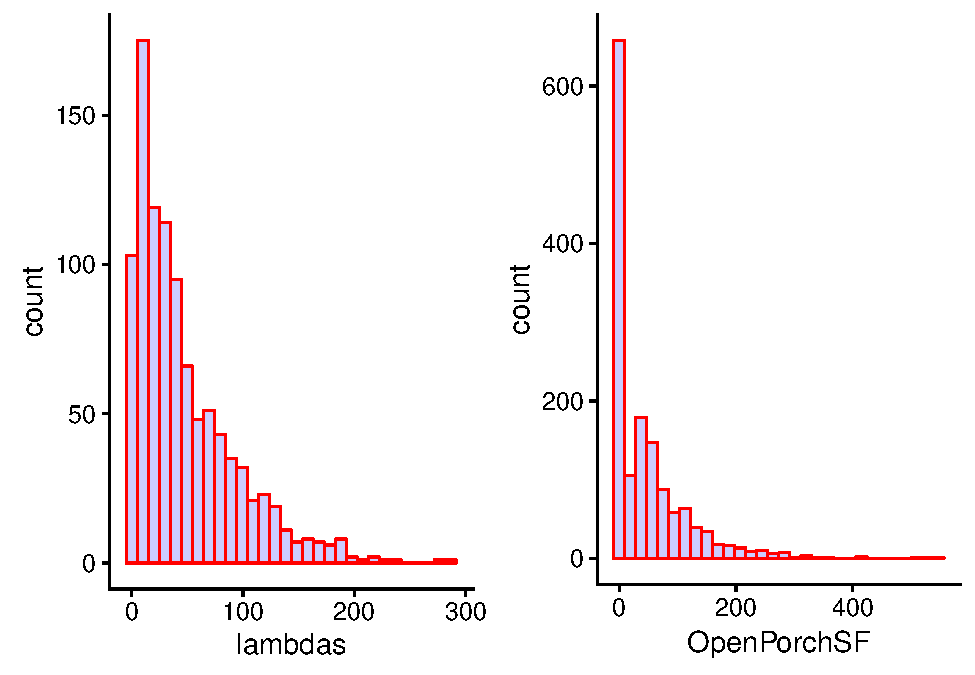
\includegraphics{DATA_605_Final_Exam_files/figure-latex/lambda-plot-1.pdf}

\href{https://en.wikipedia.org/wiki/Exponential_distribution\#Quantiles}{From
Wikipedia}, the Cumulative Distribution Function for the Exponential
Distribution is:

\[
F(x;\lambda) = 1 - e^{-\lambda x}
\]

The quantile function is thus

\[
F^{-1}(p;\lambda) = \frac{-\ln(1 - p)}{\lambda}, \ \ \ \ 0 \leq p < 1
\]

\begin{verbatim}
## [1] "5th Percentile of simulated data = 2.39336429840992"
## [1] "95th Percentile of simulated data = 139.781988205825"
## [1] "5th Percentile of empirical data = 1e-04"
## [1] "95th Percentile of empirical data = 175.0501"
\end{verbatim}

The formula for a confidence interval on normally distributed data is \[
x \pm t_{\frac{\sigma}{2}, n-1}\cdot \frac{s}{\sqrt{n}}
\]

The Z-value for a 95\% confidence interval is 1.96.

\begin{verbatim}
## [1] "95% Confidence interval for empirical data = (43.2617349622305, 50.059012982975)"
\end{verbatim}

5\% of houses in the sample have an \texttt{OpenPorchSF} value of less
than 0.0001\$, while 95\% are below 175.0501. ~ The 95\% confidence
interval tells us that with each sampling of the population (house
prices), we are 95\% sure the mean will be between
\textasciitilde{}43.26 and \textasciitilde{}50.06. ~ Due to the large
difference in percentile values between the sampled and empirical data,
the exponential distribution may not be the best fit for our dataset.

\hypertarget{modeling.}{%
\section{6. Modeling.}\label{modeling.}}

Build some type of multiple regression model and submit your model to
the competition board. Provide your complete model summary and results
with analysis. Report your Kaggle.com user name and score.

\begin{verbatim}
##            Id    MSSubClass      MSZoning   LotFrontage       LotArea 
##             0             0             0           259             0 
##        Street         Alley      LotShape   LandContour     Utilities 
##             0          1369             0             0             0 
##     LotConfig     LandSlope  Neighborhood    Condition1    Condition2 
##             0             0             0             0             0 
##      BldgType    HouseStyle   OverallQual   OverallCond     YearBuilt 
##             0             0             0             0             0 
##  YearRemodAdd     RoofStyle      RoofMatl   Exterior1st   Exterior2nd 
##             0             0             0             0             0 
##    MasVnrType    MasVnrArea     ExterQual     ExterCond    Foundation 
##             8             8             0             0             0 
##      BsmtQual      BsmtCond  BsmtExposure  BsmtFinType1    BsmtFinSF1 
##            37            37            38            37             0 
##  BsmtFinType2    BsmtFinSF2     BsmtUnfSF   TotalBsmtSF       Heating 
##            38             0             0             0             0 
##     HeatingQC    CentralAir    Electrical    firstFlrSF      secFlrSF 
##             0             0             1             0             0 
##  LowQualFinSF     GrLivArea  BsmtFullBath  BsmtHalfBath      FullBath 
##             0             0             0             0             0 
##      HalfBath  BedroomAbvGr  KitchenAbvGr   KitchenQual  TotRmsAbvGrd 
##             0             0             0             0             0 
##    Functional    Fireplaces   FireplaceQu    GarageType   GarageYrBlt 
##             0             0           690            81            81 
##  GarageFinish    GarageCars    GarageArea    GarageQual    GarageCond 
##            81             0             0            81            81 
##    PavedDrive    WoodDeckSF   OpenPorchSF EnclosedPorch threeSsnPorch 
##             0             0             0             0             0 
##   ScreenPorch      PoolArea        PoolQC         Fence   MiscFeature 
##             0             0          1453          1179          1406 
##       MiscVal        MoSold        YrSold      SaleType SaleCondition 
##             0             0             0             0             0 
##     SalePrice 
##             0
\end{verbatim}

There are many variables that can be recoded. Many columns can be
converted from numeric to categorical (factor). Some columns, especially
those with a high number of missing values, can be converted to factors
with two levels - those with the property, and those without it (1 and
0). This will allow us to still use the variable, and not have to
discard it. Lastly, we can convert four columns containing quality
information to ordered factors.

I won't be imputing any data in this model, since I believe the NAs are
not due to missing data, but rather indicate that the property does not
have that quality. For example, an NA in the \texttt{PoolQC} column
probably means that the house doesn't have a pool.

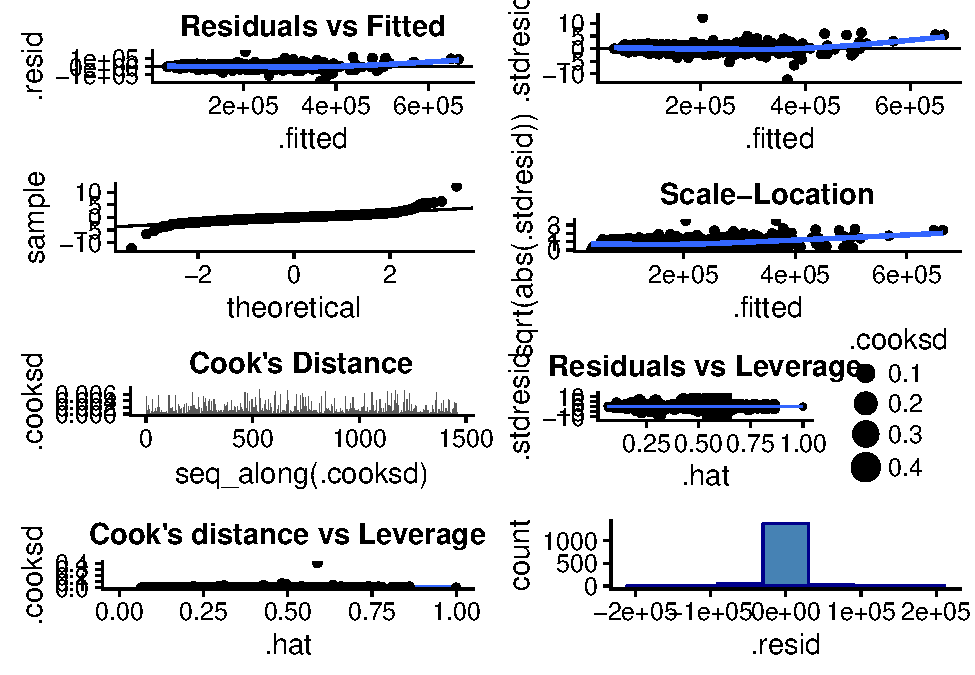
\includegraphics{DATA_605_Final_Exam_files/figure-latex/model-plots-1.pdf}

\begin{verbatim}
##    ID Predicted
## 1   1  112738.1
## 2   2  159855.4
## 3   3  199412.6
## 4   4  200603.6
## 5   5  194311.2
## 6   6  162449.4
## 7   7  173211.2
## 8   8  155506.3
## 9   9  185514.1
## 10 10  119749.0
\end{verbatim}


\end{document}
